\chapter{Methodology}

In this chapter it is going to be explained all the steps required to achieve a functional neural network to participate at the ActivityNet Challenge. For this challenge there was no baseline because video tasks have not been faced on the group I did this project, so was required to face the challenge from zero.

\section{ActivityNet Dataset}

The ActivityNet Dataset\cite{caba2015activitynet} is \textit{A Large-Scale Video Benchmark for
Human Activity Understanding}. This dataset, on version 1.3 which is the one used for the challenge, contains 19,994 videos with a different 200 activities labeled which represents a wide range of human activities. In total there are 660 hours of video and the subsets are split on the following way: 50\% training dataset, 25\% validation dataset and 25\% testing dataset. Each video of the dataset have an activity happening in there and one or more annotations saying in which temporal locations the activity is happening.

All the video from this dataset are placed on \textit{YouTube} so only the links for the video are provided because of copyright issues. So the first task to be done was download all the videos on our own. This was done using a program called \textit{youtube-dl} which allows to download videos from that platform. But some videos show up with some issues as all of them were stored on a third party platform. This issues went from some of them presenting location restrictions to some of them  even were removed by their owners. This let only download 19,811 video which considering the size of the dataset, was not a big deal.

Once all the videos from the dataset were downloaded, the number of frames of each video was extracted because the temporal unit at the time to process it will be the frames. In addition to this, some stats were computed. Such as the whole number of frames from all the videos in the dataset which is 65.6 million frames. Also, the lenght in minutes of each activity at the dataset was plot on Figure~\ref{fig:dataset_stats} to have an idea about the activities frequencies. As can be seen, not all the activities have the same appearance along the dataset, varying from 40 minutes the least frequent activity to 3.5 hours the more frequent one. In total over all the dataset there are 313 hours of activities which will be required to detect and localize.

\begin{figure}
\begin{center}
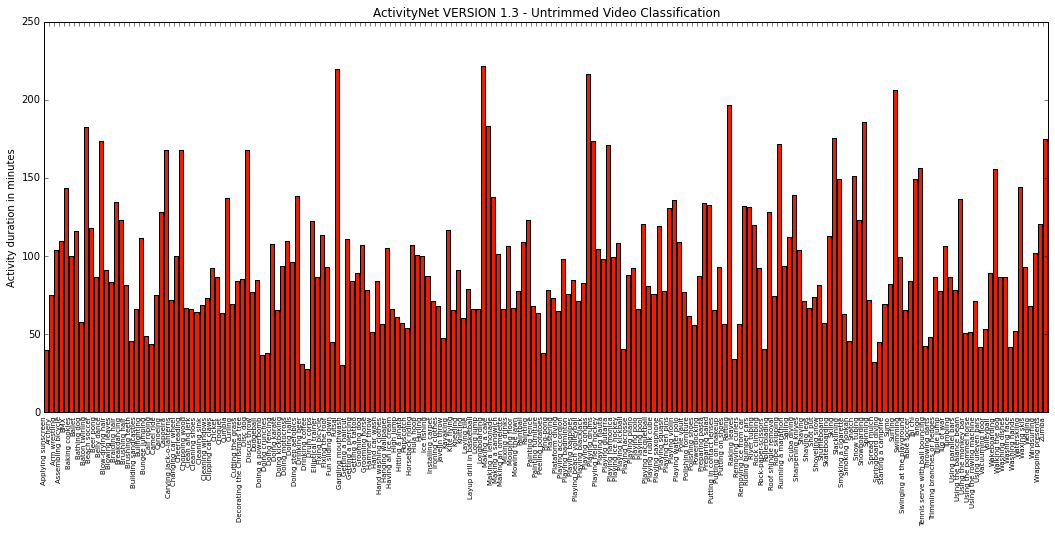
\includegraphics[width=1\linewidth]{img/methodology/dataset_stats}
\end{center}
\caption{Activity duration in minutes for each activity on the dataset}
\label{fig:dataset_stats}
\end{figure}

\section{Extracting Video Features Using C3D}

The C3D network\cite{tran2014learning} was decided to use as a video features extractor to be known to extract very well either spatial and temporal correlations from videos.
%%TODO add references

The original paper proposing and studying 3D convolutions applied to videos, also give code to reproduce it. The code given was based on a version of \textit{Caffe}\cite{jia2014caffe} dated to 2014. Because the code to use 3D convolutions did not support last functionalities and did not work with the \textit{Python} environment used for this project, the model trained with C3D and the Sports1M dataset was ported to \textit{Keras}\footnote{All the process has been open sourced and can be found in: \url{https://gist.github.com/albertomontesg/d8b21a179c1e6cca0480ebdf292c34d2}}. Keras is a deep learning framework that works over \textit{Theano}\cite{theano2016theano} and \textit{TensorFlow}\cite{abadi2016tensorflow}, two computational frameworks which allow run and train deep learning models over either CPU and GPU.

At the time to run the C3D model on the model ported to \textit{Keras}, some little changes where required to do over the source code\footnote{The fork of \textit{Keras} used can be found in: \url{https://github.com/albertomontesg/keras/tree/develop}} due to the implementation of the 3D convolution and 3D pooling operations. Once this was fixed, all the videos where passed throught the C3D model, and its features at \textit{fc6} extracted. This process could be done in parallel with 2 GPUs computing the features and multiple CPU cores fetching from disk all the videos. This task was expected to last a lot of time (one week approximately) but thanks to parallelize the process, only in two days all the features where computed from the 65.6 million frames available at the dataset.

In the process of fetching the videos from disk, was used \textit{OpenCV}\cite{opencv_library} a framework with interesting utils fot Computer Vision applications. With this software, the videos were read in chunks of 16 frames, resized to 112x112 as input frame size and then feed the C3D network. The output of the model, a sequence of 4096-sized vectors where stored in disk for preparing it to train the Recurrent Neural Network.

\section{Extracting Audio Features}

The audio features extracted: MFCC and Spectral

%%TODO: Ask for bibliografy

\section{Prepare the Data for Stateful Recurrent Networks}

Since all the videos on the ActivityNet Dataset are not from the same length, to train a recurrent neural network, it requires to give it a fixed lenght sequence. This length is called \textit{timestep} and must be a value not very high because as the gradient propagates along all the sequence, if the timestep is very high, the gradient might achieve very high values known as \textit{exploting gradient}.

There are two main solutions to this, in order to keep the memory state of the LSTM cells for a long sequences. The first solution would require to clip it as is explained in \cite{pascanu2012difficulty}. The second solution is to train the Recurrent Neural Network without reseting the memory between each batch. With this approach, if a video sequence longer than the \textit{timestep} does not fit into the batch, the RNN can be trained passing framents of the videos one after the other at the same batch position, and because the memory is not reset after each batch, at the training of the next batch, the memory will be preserve. For this configuration the different videos must be carefully set on the same batch index to exploit the \textit{Keras} functionality of stateful training for RNNs.





How the data was prepared to be trained to the Recurrent Network

\section{Networks Configuration}

Talk about the different configurations I have tried:
\begin{itemize}
    \item Normal LSTM with different variations in number of layers and neurons
    \item Feedback Model
    \item Semisupervised
\end{itemize}

\section{Post-Processing Proposed}

How to compute the classification for each video.

How to get the temporal localization of the activities to the videos.
Mean filter, activity probability computation.
